\chapter{Γενική Δομή Αρχιτεκτονικής}
\label{chap:Arch}

\section{Επίπεδα Συστήματος}

Με οδηγό το υπηρεσιοκεντρικό μοντέλο που περιγράφηκε στην ενότητα
\ref{sec:SOA}, το σύστημα δομείται σε αρχιτεκτονικά επίπεδα. Όπως 
αναφέρθηκε ένα SOA σύστημα χωρίζεται σε:

\newcounter{numberedCntA}
\begin{enumerate}
\item \textbf{Presentation.} Αφορά εφαρμογές που χρησιμοποιούν το σύστημα.
\item \textbf{Business Process.} Εκτελεί συγκεκριμένη λειτουργία που 
έχει να κάνει με τον τύπο της εφαρμογής και συντίθεται από τις 
υπάρχουσες υπηρεσίες.
\item \textbf{Services.} Συμπεριλαμβάνει όλες τις υπηρεσίες.
\item \textbf{Enterprise.} Εξυπηρετεί απευθείας τις ανάγκες των 
υπηρεσιών και προσφέρει πρόσβαση στα συστήματα της επιχείρησης.
\item \textbf{Operational Systems.} Αποτελείται από τις υπάρχουσα 
εμπορικά και μη εξωτερικά συστήματα ή κάποιο συνδυασμό αυτών.
\setcounter{numberedCntA}{\theenumi}
\end{enumerate}

\begin{figure}[htbp]
  \begin{center}
    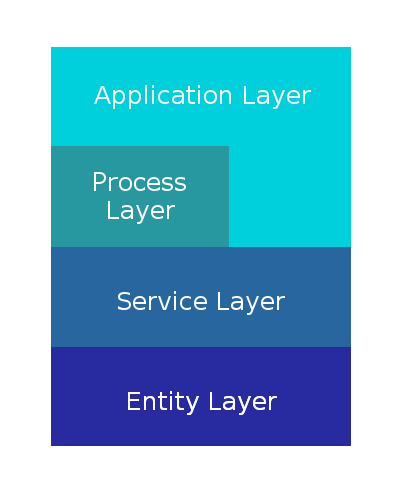
\includegraphics[scale=0.35]{Figures/Architecture/Layers.png}
  \end{center}
  \caption{Τα επίπεδα της αρχιτεκτονικής}
  \label{fig:Layers}
\end{figure}

Με βάση την παραπάνω κατηγοριοποίηση το σύστημα χωρίζεται σε τέσσερα 
επίπεδα. Ξεκινώντας από την κορυφή όπως φαίνεται στο σχήμα 
\ref{fig:Layers} έχουμε:

\begin{itemize}
\item \textbf{Επίπεδο Εφαρμογής (Application Layer).} Το επίπεδο αυτό 
περιλαμβάνει την λογική οποιασδήποτε εφαρμογής που χρησιμοποιήσει την 
παρούσα αρχιτεκτονική. Δεν αφορά την προκείμενη αρχιτεκτονική.
\item \textbf{Επίπεδο Διαδικασιών (Process Layer).} Το επίπεδο αυτό 
περιέχει όλες τις διαδικασίες που στην ουσία είναι συνδυασμός υπηρεσιών 
ώστε να παράγουν ουσιώδεις λειτουργίες προς διευκόλυνση της ανάπτυξης 
εφαρμογών. Στην ουσία οι διαδικασίες είναι κι αυτές υπηρεσίες.
\item \textbf{Επίπεδο Υπηρεσιών (Service Layer).} Το επίπεδο των 
υπηρεσιών περιλαμβάνει ένα σύνολο από διαφορετικές υπηρεσίες. Με τον όρο 
υπηρεσία (service) αναφερόμαστε σε όλες τις σαφώς οριζόμενες και 
αυτόνομες λειτουργίες που έχουν νόημα για ένα peer-to-peer σύστημα. 
Είναι στην ουσία αναπαράσταση αλγορίθμων, πρωτοκόλλων και 
λειτουργικότητας που προσφέρει το σύστημα. Μπορούμε να το δούμε ως μια 
ενέργεια που επιδρά πάνω στο επίπεδο των οντοτήτων. Απόρροια αυτού 
μπορεί να είναι η ανανέωση της αποθηκευμένης πληροφορίας όχι μόνο τοπικά 
σε κάποιον peer αλλά και συνολικά στο σύστημα. Μπορεί να οδηγήσει στην 
αλλαγή της κατάστασης του τοπικού peer ακόμα και μέρους του δικτύου. 
Επίσης, μπορεί να επιστρέψει χρήσιμες πληροφορίες για το σύστημα ή για 
τα δεδομένα που αποθηκεύονται σε αυτό. Η υπηρεσία είναι το δομικό 
στοιχείο της αρχιτεκτονικής βάσει της οποίας ο χρήστης μπορεί είτε να 
δομήσει την εφαρμογή του είτε να προσθέσει επιπλέον λειτουργικότητα στο 
σύστημα.
\item \textbf{Επίπεδο Οντοτήτων (Entity Layer).} Το επίπεδο των 
οντοτήτων είναι το κατώτερο επίπεδο της αρχιτεκτονικής πάνω στο οποίο 
επιδρούν και στηρίζονται όλα τα υπόλοιπα. Με τον όρο οντότητα ονομάζουμε 
όλα τα αντικείμενα τα οποία διατηρούν κατάσταση ή μπορούν να προσφέρουν 
πρόσβαση σε πόρους του συστήματος. Επίσης συμπεριλαμβάνονται και αυτά 
που προσφέρουν λειτουργικότητα από το λειτουργικό σύστημα στο οποίο 
τρέχει η εφαρμογή. Παράδειγμα είναι η ικανότητα επικοινωνίας με άλλες 
εφαρμογές μέσω απομακρυσμένων κλήσεων συναρτήσεων (rpc) ή με τη χρήση 
socket.
\end{itemize}

\section{Σχεδιαστικό Πρότυπο Dependency Injection}

\subsection{Εξήγηση προτύπου}

Η αρχιτεκτονική έχει χωριστεί σε διακριτά επίπεδα. Κάθε επίπεδο περιέχει 
τα δικά του domain object τα οποία ενθυλακώνουν σαφώς ορισμένη και 
ξεχωριστή λειτουργικότητα \citep{POSA4}. Αυτά κατηγοριοποιούνται 
σε περισσότερο, δυο όμως συμπίπτουν με την παρούσα αρχιτεκτονική. Αυτά 
είναι το application service το οποίο έχει την ίδια έννοια με την 
υπηρεσία όπως έχει οριστεί εδώ και το component το οποίο αντιστοιχεί 
στις οντότητες του επιπέδου οντοτήτων όπως περιγράφηκε. Όλα αυτά θέτουν 
κάποια κοινά προβλήματα, όπως ο τρόπος σύνδεσης διεπαφών και 
υλοποιήσεων, ο τρόπος που θα κατασκευάζονται, ο έλεγχος του κύκλου ζωής 
και η παραμετροποίηση τους είτε κατά την εκκίνηση του συστήματος είτε 
κατά τον χρόνο εκτέλεσης. Λύσεις σε αυτά τα ζητήματα δίνονται μεμονωμένα 
από διάφορα σχεδιαστικά πρότυπα. Παρακάτω δικαιολογείται η επιλογή του 
σχεδιαστικού προτύπου Dependency Injection \citep{Fowler2004} για την λύση 
των παραπάνω ζητημάτων στο σύνολό τους.

Μια κλάση μπορεί να χρησιμοποιεί διάφορες διεπαφές οι οποίες με τη σειρά 
τους έχουν κάποιες υλοποιήσεις. Η βασική ιδέα του σχεδιαστικού προτύπου 
dependency injection είναι η ύπαρξη ενός ξεχωριστού αντικειμένου που 
είναι υπεύθυνο να προσφέρει στις κλάσεις υλοποιήσεις των διεπαφών που 
χρησιμοποιεί. Προγραμματιστικά σημαίνει πως η κλάση δεν περιέχει κώδικα 
που αρχικοποιεί αντικείμενα από τα οποία εξαρτάται. Η λειτουργία αυτή 
έχει μεταφερθεί στο ξεχωριστό αντικείμενο που αναφέρθηκε το οποίο 
ονομάζεται dependency injector. Το αποτέλεσμα που προκύπτει είναι η 
αφαίρεση των εξαρτήσεων από τις υλοποιήσεις των διεπαφών που 
χρησιμοποιεί μια κλάση. Οι εξαρτήσεις πλέον γίνονται εμφανείς ως 
ορίσματα στον constructor ή σε μεθόδους που αρχικοποιούν τα πεδία τις 
κλάσης (getter/setter μέθοδοι). Ο injector, επομένως, κατασκευάζει το 
ζητούμενο αντικείμενο ικανοποιώντας όλες τις εξαρτήσεις του.

Αντίστοιχη λύση μπορεί να δοθεί και από το σχεδιαστικό πρότυπο Service 
Locator \citep{dan2003core} που είναι μια παραλλαγή του 
προτύπου Inversion of Control. Παρέχεται ένα γενικό σημείο πρόσβασης 
προς όλες τις υπηρεσίες χωρίς να ενδιαφέρει η υλοποίηση που 
χρησιμοποιείται και ο τρόπος με τον οποίο αναζητείται από τον service 
locator. Η διαφορά και το μειονέκτημα σε σύγκριση με το πρότυπο 
Dependency Injection είναι πως η μοναδική εξάρτηση που έχει πλέον μια 
κλάση είναι το αντικείμενο service locator.

Λαμβάνουμε διάφορα οφέλη από την χρήση του σχεδιαστικού προτύπου 
Dependency Injection. Ο κώδικας χωρίζεται σε ευδιάκριτες μονάδες 
(module) και έχουμε πλήρη διαχωρισμό διεπαφών και υλοποιήσεων. Οι 
κλάσεις δεν γνωρίζουν τίποτα για τις υλοποιήσεις των διεπαφών που 
χρησιμοποιούν. Διαχωρίζεται δηλαδή, η συμπεριφορά και η λειτουργικότητα 
που προσφέρεται από την λύση των εξαρτήσεων. Επίσης γίνεται περισσότερο 
επαναχρησιμοποιήσιμος (reusable) και είναι πιο ευανάγνωστος αφού οι 
εξαρτήσεις είναι ορατές. Τέλος, διευκολύνεται ο έλεγχος ορθής 
λειτουργίας του κώδικα όπως η χρήση Mock Object \citep{Freeman04mockroles} 
το οποίο παρέχεται στη θέση μιας πραγματικής υλοποίησης μιας διεπαφής από την 
οποία εξαρτάται η κλάση.

\subsection{Guice}

Στην υλοποίηση της βιβλιοθήκης χρησιμοποιήθηκε η Guice, ένα ελαφρύ 
πλαίσιο που υλοποιεί το πρότυπο dependency injection για την Java 
κατασκευασμένο από την Google. Όλες οι πληροφορίες παραμετροποίησης των 
συνδέσεων μεταξύ διεπαφών και υλοποιήσεων περιέχονται κυρίως σε ένα 
Module. Γενικά μια εφαρμογή που ακολουθεί αυτό το πρότυπο αποτελείται 
από διάφορα module και κώδικα που αφορά την αρχικοποίηση της.

\begin{wrapfigure}{L}{0.5\textwidth}
  \begin{center}
    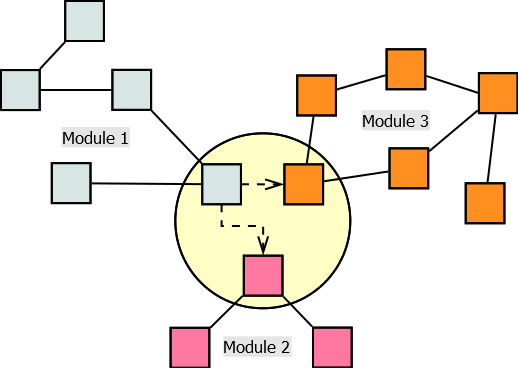
\includegraphics[width=0.48\textwidth]{Figures/Guice_modules.png}
  \end{center}
  \caption{Σύνθεση module μέσω της Guice}
  \label{fig:Guice}
\end{wrapfigure}

Η κλάση που είναι υπεύθυνη για την κατασκευή των αντικειμένων είναι ο 
Injector. Για την αρχικοποίηση του χρειάζονται τα module. Σε γενικές 
γραμμές, όταν ζητηθεί η κατασκευή ενός αντικειμένου ενός τύπου, αρχικά 
βρίσκει τι να κατασκευάσει αφού μπορεί να υπάρχουν πολλές υλοποιήσεις. 
Στη συνέχεια λύνει τις εξαρτήσεις και αρχικοποιεί το αντικείμενο.

Κατά την εκκίνηση του συστήματος, όλη η παραμετροποίηση του όσον αφορά 
τι υλοποιήσεις θα χρησιμοποιηθούν παρέχεται από τα module όπως 
περιγράφηκε. Επιπλέον, έχουμε τη δυνατότητα αλλαγών κατά τη διάρκεια 
εκτέλεσης (runtime) του προγράμματος.

Ένα άλλο σημαντικό ζήτημα είναι και ο κύκλος ζωής των αντικειμένων που 
παράγονται. Αυτός ελέγχεται από τα λεγόμενα Scope. Αυτά περιγράφουν πόσο 
θα ζήσει ένα αντικείμενο κι αν είναι σε θέση να επαναχρησιμοποιηθεί. Οι 
λόγοι είναι επειδή είτε κρατάνε κατάσταση, είτε είναι ακριβά στην 
κατασκευή ή στη διατήρηση τους. Στην Guice προσφέρονται κάποια έτοιμα, 
τα οποία φαίνονται παρακάτω, αλλά παρέχεται και όλο το πλαίσιο να 
υλοποιηθούν νέα με την απαραίτητη λειτουργικότητα.

\newcounter{numberedCntE}
\begin{enumerate}
\item Unscoped: Το αντικείμενο παράγεται εκ νέου μετά από κάθε αίτηση 
κατασκευής στον injector.
\item Singleton: Το αντικείμενο που επιστρέφει ο injector είναι το ίδιο 
για όλη την εφαρμογή.
\item RequestScoped: Το αντικείμενο διαρκεί για μια web/rpc αίτηση 
(αφορά web εφαρμογές και servlet).
\item SessionScoped: Το αντικείμενο διαρκεί για μια HTTP συνεδρία. 
(αφορά web εφαρμογές και servlet).
\setcounter{numberedCntE}{\theenumi}
\end{enumerate}

\section{Δομή Υπηρεσίας}

Πλέον έχουμε την κατάλληλη βάση για την περιγραφή της δομής της 
υπηρεσίας που εισάγει η παρούσα αρχιτεκτονική. Οι αρχές που διέπουν τις 
υπηρεσίες και αναφέρθηκαν στην περιγραφή των υπηρεσιοκεντρικών 
συστημάτων είναι σημαντικό να εφαρμοστούν και στην παρούσα 
αρχιτεκτονική. Είναι απαραίτητο να υπάρχει μια ενιαία δομή αφού αυτό 
επιβάλλει μια ομοιομορφία στο επίπεδο. Το αποτέλεσμα είναι οι διάφορες 
υπηρεσίες να είναι εύκολα κατανοητές και το πιο σημαντικό είναι η 
ανάπτυξη ενός πλάνου για την υλοποίηση ή την τροποποίηση αυτών. Στο σχήμα 
\ref{fig:ServiceStructure} φαίνεται η δομή και ακολουθεί η εξήγηση καθώς και η 
αιτιολόγηση της ύπαρξής των στοιχείων από τα οποία αποτελείται. 

Να σημειωθεί πως για την κλήση απομακρυσμένων συναρτήσεων έχει 
χρησιμοποιηθεί η CORBA και προσθέτοντας κάποιες απαιτήσεις όσον αφορά 
την δομή της υπηρεσίας. Αυτό δε μας περιορίζει στο να αντικατασταθεί με 
κάποια άλλη βιβλιοθήκη. Οι αλλαγές που θα προκύψουν θα έχουν να κάνουν 
μόνο με τις διεπαφές και τις κλάσεις της CORBA.

\begin{figure}[htbp]
  \begin{center}
    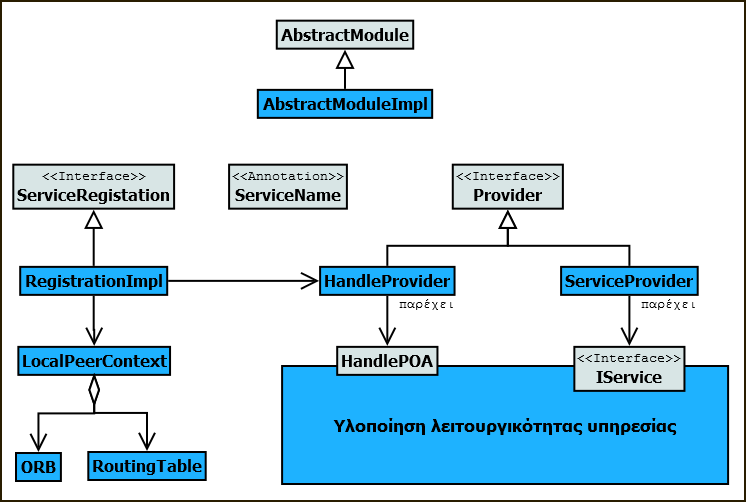
\includegraphics[width=0.95\textwidth]{Figures/Architecture/General_service_structure.png}
  \end{center}
  \caption{Γενική δομή υπηρεσίας}
  \label{fig:ServiceStructure}
\end{figure}

\paragraph{Διεπαφή Υπηρεσίας.} Όπως αναφέρθηκε στην ανάλυση των 
SOA συστημάτων, η υπηρεσία προσφέρει πρόσβαση στον χρήστη σε μια ή 
περισσότερες λειτουργίες. Είναι φυσικό να υπάρχει η διεπαφή που καθορίζει 
τις ενέργειες που μπορούν να γίνουν. Μέσω αυτής της διεπαφής πρέπει να 
περιγράφεται όλο εκείνο το πλαίσιο στο οποίο εκτελείται η υπηρεσία 
εννοώντας τους περιορισμούς που τίθενται. Η διεπαφή IService του σχήματος 
\ref{fig:ServiceStructure} αντιπροσωπεύει μια τέτοια διεπαφή. Γύρω από αυτήν 
μπορεί να υπάρξουν και άλλες βοηθητικές κλάσεις ή διεπαφές. Για παράδειγμα 
είναι πιθανό κατά την εκτέλεση μιας υπηρεσίας να αλλάξει μονοπάτι ο peer. 
Αυτή η πληροφορία μπορεί να αφορά άμεσα την εφαρμογή και θα πρέπει ως 
αποτέλεσμα να υπάρξει συγκεκριμένη αντίδραση. Το πρόβλημα αυτό λύνεται 
με το σχεδιαστικό πρότυπο Observer \citep{GoF} ή Listener όπως ονομάζεται 
αλλιώς στον κόσμο της Java.

\paragraph{Java IDL (Servant).} Η δυνατότητα εκτέλεσης της υπηρεσίας ως 
απομακρυσμένης κλήσης συνάρτησης (rpc) ικανοποιείται από την CORBA. Κατ' 
επέκταση είναι αναγκαία η περιγραφή της υπηρεσίας σε IDL. Από αυτήν 
παράγονται οι απαραίτητοι τύποι. Ανάμεσα σε αυτούς είναι και ο Servant 
%$[$παραπομπή$]$ 
ο οποίος παρέχει την ίδια λειτουργικότητα με την 
υπηρεσία. Είναι εκείνο το αντικείμενο που θα κληθεί όταν ένας peer λάβει 
μια αίτηση εκτέλεσης της υπηρεσίας.

\paragraph{Διεπαφή Provider.} Η κατασκευή αντικειμένων των υλοποιήσεων είτε 
της υπηρεσίας είτε του Servant μπορεί να είναι μια πολύπλοκη διαδικασία 
η οποία δε θα έπρεπε να απασχολεί τον χρήστη. Στην προκειμένη περίπτωση, 
η Guice έχει αναλάβει την κατασκευή τους. Οι κλάσεις που υλοποιούν την 
διεπαφή Provider είναι ικανές να παρέχουν συγκεκριμένα αντικείμενα. 
Περιγράφουν στην Guice τον τρόπο με τον οποίο κατασκευάζονται πολύπλοκοι 
τύποι. Επίσης, μέσω των Provider μπορούμε να ελέγξουμε τον κύκλο ζωής 
τον αντικειμένων που επιστρέφει. Παράδειγμα η υλοποίηση του Servant δεν 
έχει νόημα να κατασκευάζεται συνεχώς εκ νέου. Έχει επιλεχθεί επομένως ο 
Provider του να συμπεριφέρεται ως singleton και έτσι να επιστρέφει το 
ίδιο αντικείμενο όταν του ζητείται. Σε αντίθεση με την υλοποίηση της 
διεπαφής της υπηρεσίας όπου εκεί μπορούμε να κατασκευάζουμε νέο κάθε 
φορά. Βέβαια υπάρχουν και περιπτώσεις όπου, όπως περιγράφηκε στην 
ενότητα του Dependency Injection, μπορεί να είναι ακριβό η συνεχής 
κατασκευή.

\paragraph{Εγκατάσταση υπηρεσίας.} Τον χρήστη της υπηρεσίας δεν τον 
απασχολεί ο τρόπος με τον οποίο ένας peer ξεκινά να εξυπηρετεί 
απομακρυσμένες αιτήσεις μιας υπηρεσίας. Αυτό καλύπτεται από την διεπαφή 
ServiceRegistration. Στην παρούσα φάση όπου εξαρτόμαστε από την CORBA, 
τα βήματα είναι η δημιουργία ενός Servant της υπηρεσίας που θέλουμε και 
η εγκατάστασή του στον POA. Για να επιτευχθεί αυτό χρειάζεται μια 
αναφορά προς το ORB του peer. Αυτή μπορεί να ληφθεί μέσω του 
LocalPeerContext που κρατά πληροφορίες για τον τοπικό peer, αναφορές 
προς τον πίνακα δρομολόγησης του και το ORB του.

Η διεπαφή ServiceRegistration πρόκειται να έχει τόσες υλοποιήσεις όσες 
και οι υπηρεσίες του συστήματος. Είναι αναγκαίος ένας τρόπος ώστε η 
Guice να ξέρει ποια να επιστρέφει όταν ζητείται μιας συγκεκριμένης 
υπηρεσίας. Αυτό επιτυγχάνεται με τη δημιουργία ενός annotation. Στην 
εικόνα \ref{fig:ServiceStructure} το ServiceName παίζει αυτόν τον ρόλο.

\paragraph{Λειτουργικότητα Υπηρεσίας.} Μετά τον καθορισμό των παραπάνω 
έχουμε την υλοποίηση της υπηρεσίας όπου προσφέρεται η λειτουργικότητά της. 
Εδώ έχουμε τον χώρο για την δήλωση όλων των βοηθητικών διεπαφών και κλάσεων 
καθώς και των υλοποιήσεών του. Είναι προφανές πως η λογική που θα 
ακολουθηθεί εδώ κρίνει και κατά πόσο η υπηρεσία θα καταστεί επεκτάσιμη 
και τροποποιήσιμη. Στην εικόνα \ref{fig:ServiceStructure} φαίνεται αυτό 
το κομμάτι καθώς και οι διεπαφές που το καλύπτουν.

\paragraph{Παραμετροποίηση Module.} Τελικά, καταλήγουμε να έχουμε υλοποιήσεις όλων 
των αναγκαίων κλάσεων και διεπαφών καθώς και εκείνου του κομματιού που 
έχει σχέση με την αυτή καθεαυτή λειτουργικότητα της υπηρεσίας. Αυτό που 
απομένει είναι η δήλωση όλων των αντιστοιχίσεων διεπαφών/κλάσεων με τις 
υλοποιήσεις τους ώστε να γνωρίζει η Guice τον τρόπο με τον οποίο θα 
παράγει αντικείμενα αυτών λύνοντας τις εξαρτήσεις τους. Η υλοποίηση της 
κλάσης AbstractModule που προσφέρεται από την Guice εξυπηρετεί αυτόν τον 
σκοπό. Να σημειωθεί πως μπορεί να έχουμε αρκετές υλοποιήσεις της ίδιας 
υπηρεσίας. Κατά την εκκίνηση του προγράμματος θα έχουμε μια συσχέτιση με 
συγκεκριμένη υλοποίηση. Παρόλα αυτά μπορεί να είναι αναγκαίο κατά τον 
χρόνο εκτέλεσης του συστήματος να γίνει αλλαγή σε άλλη υλοποίηση της 
υπηρεσίας. Η συμπεριφορά αυτή δηλώνεται στο Module ως multibindings όσον 
αφορά τον τρόπο με τον οποίο το επιτυγχάνει η Guice.

\section{Δομή Διαδικασιών}

\begin{figure}[htbp]
  \begin{center}
    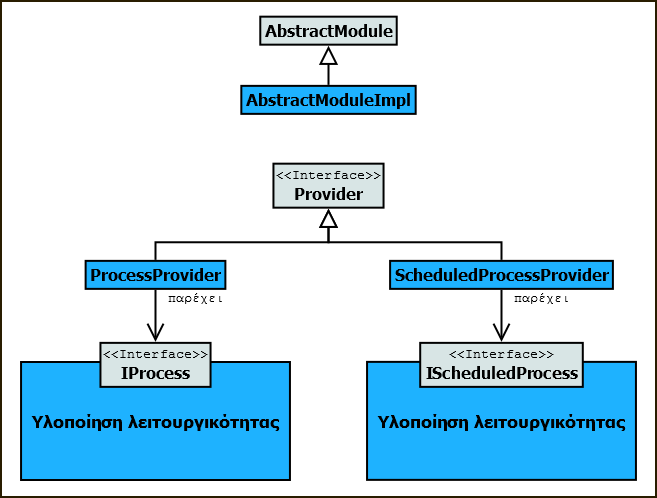
\includegraphics[width=0.95\textwidth]{Figures/Architecture/General_process_structure.png}
  \end{center}
  \caption{Γενική δομή διαδικασίας}
  \label{fig:ProcessStructure}
\end{figure}

Όπως αναφέρθηκε η διαδικασία είναι αποτέλεσμα της σύνθεσης 
διάφορων υπηρεσιών. Στόχος είναι να παραχθεί λειτουργικότητα που έχει 
νόημα και είναι χρήσιμη στην εφαρμογή. Στην ουσία η διαδικασία είναι και 
αυτή ένας τύπος υπηρεσίας.Εδώ υπάρχει μεγαλύτερη ελευθερία αφού 
εδώ η γενική δομή που απεικονίζεται στο σχήμα \ref{fig:ProcessStructure} 
είναι απλά ενδεικτική.

\paragraph{Διεπαφή διαδικασίας.} Η περιγραφή της λειτουργικότητας και των 
περιορισμών που θέτει η διαδικασία γίνεται μέσω της διεπαφής της.

\paragraph{Provider.} Όπως και στις υπηρεσίες, έτσι κι εδώ, μια διαδικασία 
μπορεί να είναι πολύπλοκη στην κατασκευή. Ένας Provider αναλαμβάνει να 
κατασκευάσει τέτοια αντικείμενα αποκρύπτοντας τον τρόπο από τον χρήστη.

\paragraph{Παραμετροποίηση Module.} Αντίστοιχα, οι αντιστοιχίσεις 
διεπαφών/κλάσεων με τις υλοποιήσεις τους που αφορούν την Guice 
βρίσκονται στο Module της διαδικασίας.

Πέρα από την απλή σύνθεση των διαδικασιών, μπορούν να εισαχθούν 
νέες έννοιες (semantics). Στην παρούσα φάση, πέρα από την απλή, έχουμε 
την έννοια της προγραμματιζόμενης διαδικασίας. Για να γίνει μια 
διαδικασία προγραμματισμένη ώστε να εκτελείται ανά τακτά χρονικά 
διαστήματα, πρέπει να υλοποιηθεί η κλάση TimerTask της Java. Όσον αφορά 
την Guice, για τον διαχωρισμό τον υλοποιήσεων, χρειάζεται η ανάγκη ενός 
annotation που να δηλώνει την παραπάνω έννοια.
